% THIS DOCUMENT IS FOLLOWS THE VOLERE TEMPLATE BY Suzanne Robertson and James Robertson
% ONLY THE SECTION HEADINGS ARE PROVIDED
%
% Initial draft from https://github.com/Dieblich/volere
%
% Risks are removed because they are covered by the Hazard Analysis
\documentclass[12pt]{article}

\usepackage{booktabs}
\usepackage{tabularx}
\usepackage{hyperref}
\usepackage{graphicx}
\usepackage{graphicx}
\usepackage{enumitem}
\hypersetup{
    bookmarks=true,         % show bookmarks bar?
      colorlinks=true,      % false: boxed links; true: colored links
    linkcolor=red,          % color of internal links (change box color with linkbordercolor)
    citecolor=green,        % color of links to bibliography
    filecolor=magenta,      % color of file links
    urlcolor=cyan           % color of external links
}

\newcommand{\lips}{\textit{Insert your content here.}}

%% Comments

\usepackage{color}

\newif\ifcomments\commentstrue %displays comments
%\newif\ifcomments\commentsfalse %so that comments do not display

\ifcomments
\newcommand{\authornote}[3]{\textcolor{#1}{[#3 ---#2]}}
\newcommand{\todo}[1]{\textcolor{red}{[TODO: #1]}}
\else
\newcommand{\authornote}[3]{}
\newcommand{\todo}[1]{}
\fi

\newcommand{\wss}[1]{\authornote{magenta}{SS}{#1}} 
\newcommand{\plt}[1]{\authornote{cyan}{TPLT}{#1}} %For explanation of the template
\newcommand{\an}[1]{\authornote{cyan}{Author}{#1}}

%% Common Parts

\newcommand{\progname}{SFWRENG 4G06 - Capstone Design Process}
\newcommand{\authname}{\textbf{Team 17, DomainX} \\
\\ Awurama Nyarko
\\ Haniye Hamidizadeh
\\ Fei Xie
\\ Ghena Hatoum             
}
\usepackage{hyperref}
    \hypersetup{colorlinks=true, linkcolor=blue, citecolor=blue, filecolor=blue,
                urlcolor=blue, unicode=false}
    \urlstyle{same}
                                


\begin{document}

\title{Software Requirements Specification for \progname: subtitle describing software} 
\author{\authname}
\date{\today}
	
\maketitle

~\newpage

\pagenumbering{roman}

\tableofcontents

~\newpage

\section*{Revision History}

\begin{tabularx}{\textwidth}{p{3cm}p{2cm}X}
\toprule {\textbf{Date}} & {\textbf{Version}} & {\textbf{Notes}}\\
\midrule
2025-10-05 & 1.0 & Added Product Boundary \\
2025-10-05 & 1.1 & Added Product Use Case Table \\
2025-10-05 & 1.2 & Added Individual Product Use Cases (PUC's) \\
2025-10-05 & 1.3 & Added Functional Requirements \\
2025-10-05 & 1.4 & Added Look and Feel Requirements \\
2025-10-05 & 1.5 & Added Usability and Performance Requirements \\
\bottomrule
\end{tabularx}

~\\

~\newpage
\section{Purpose of the Project}
\subsection{User Business}
\lips
\subsection{Goals of the Project}
\lips
\section{Stakeholders}
\subsection{Client}
\lips
\subsection{Customer}
\lips
\subsection{Other Stakeholders}
\lips
\subsection{Hands-On Users of the Project}
\lips
\subsection{Personas}
\lips
\subsection{Priorities Assigned to Users}
\lips
\subsection{User Participation}
\lips
\subsection{Maintenance Users and Service Technicians}
\lips

\section{Mandated Constraints}
\subsection{Solution Constraints}
\lips
\subsection{Implementation Environment of the Current System}
\lips
\subsection{Partner or Collaborative Applications}
\lips
\subsection{Off-the-Shelf Software}
\lips
\subsection{Anticipated Workplace Environment}
\lips
\subsection{Schedule Constraints}
\lips
\subsection{Budget Constraints}
\lips
\subsection{Enterprise Constraints}
\lips

\section{Naming Conventions and Terminology}
\subsection{Glossary of All Terms, Including Acronyms, Used by Stakeholders
involved in the Project}
\lips

\section{Relevant Facts And Assumptions}
\subsection{Relevant Facts}
\lips
\subsection{Business Rules}
\lips
\subsection{Assumptions}
\lips

\section{The Scope of the Work}
\subsection{The Current Situation}
\lips
\subsection{The Context of the Work}
\lips
\subsection{Work Partitioning}
\lips
\subsection{Specifying a Business Use Case (BUC)}
\lips

\section{Business Data Model and Data Dictionary}
\subsection{Business Data Model}
\lips
\subsection{Data Dictionary}
\lips

\section{The Scope of the Product}
\subsection{Product Boundary}
This system aims to simplify and streamline the process of collecting, managing, and analyzing data to assess the state of the practice for various research domains. It replaces the existing, manual process (currently managed via Excel sheets) and formalizes the methodology outlined in the \href{https://arxiv.org/abs/2110.11575}{Methodology for Assessing the State of the Practice for Domain X paper}. The final system will be a secure, accessible, data management and analysis tool.

The system will provide the following core functionality:
\begin{itemize}
  \item \textbf{Security and User Management:}
  \begin{itemize}
    \item Securely manage user accounts (login, password changes).
    \item Accounts can only be created by an administrator invitation.
    \item Enforce Role-Based Access Control (RBAC).
    \item Ensure only authenticated users can modify data.
  \end{itemize}
  \item \textbf{Data Integrity and Auditing:} Maintain an audit trail for all data entries, logging when a change is made.
  \item \textbf{Core Data Operations:} Facilitate the storing, updating, and retrieving of all core research entities: research domains, libraries, and collected metrics.
  \item \textbf{Data Collection:}
  \begin{itemize}
    \item Support mass data upload from previous research work.
    \item Automatically collect data to populate a specified data table (e.g., State-of-Practice Metrics Table).
  \end{itemize}
  \item \textbf{Analysis and Visualization:}
  \begin{itemize}
    \item Implement an AHP-based ranking of libraries within a domain based on their state of practice.
    \item Visualize data as different 2D graphs, showing the difference between libraries in a domain.
  \end{itemize}
  \item \textbf{User Experience (UX):}
  \begin{itemize}
    \item Have an intuitive UI to improve overall user experience.
    \item Ensure accessible read permissions for all users.
  \end{itemize}
  \item \textbf{Data Export:} Allow users to download tables or graphs onto their local device.
\end{itemize}

\noindent The following capabilities are explicitly excluded from the initial scope:

\begin{itemize}
  \item \textbf{Communication:} The system will not facilitate scheduling or hosting meetings between researchers and domain experts.
  \item \textbf{User Data:} Only username, email, and password will be collected for user profiles, no need for personal information.
  \item \textbf{Fine-Grained Permissions:} The system will not separate domain access by researcher. All authenticated researchers will be able to view and edit any domain.
  \item \textbf{Data/Library Recommendations:} The system will not give users suggestions on which library to use based on insufficient information.
  \item \textbf{Data Imputation/Handling:} The system will not automatically fill in missing data, nor will it incorporate a mechanism to assume the possibility of missing data during AHP calculation.
  \item \textbf{System Management:} The system will not include functionality for adding or removing administrator accounts.
  \item \textbf{AHP Validation:} The system will not include functionality to check the accuracy of the AHP calculations.
\end{itemize}

\noindent The following items are recognized as potential enhancements but are considered low-priority:

\begin{itemize}
  \item \textbf{Data Auditing:} Logging who edited the data entries.
  \item \textbf{Conflict Resolution:} Creating a method for merging changes when multiple users edit the same data simultaneously.
\end{itemize}

\subsection{Product Use Case Table}
\begin{tabularx}{\textwidth}{|p{2cm}|p{2cm}|p{2cm}|X|} \hline
\toprule
\textbf{Use Case (Goal)} & \textbf{Primary Actor} & \textbf{Secondary Actor(s)} & \textbf{Key Functional Requirements (FRs)} \\ \hline
\midrule
Invite New Users & Admin & Researcher & Admin can input a new user email. New user will receive an email with a link that will allow them to setup an account, password, and username. \\  \hline
Domain Creation \& Setup & Admin & Researcher & Create new Domain (must validate unique name). Optional: Add description to the domain. \\  \hline
Publish Domain & Researcher & General Users & Once the data collection is finished, allow anyone to see it (General Users). \\  \hline
Automation Library Data & Researcher & System & Auto-fill fields (e.g., creation date, commit date) upon entering a public URL. Check for and flag missing data that was expected to be collected. \\  \hline
Manually Input/Update Data & Researcher & System & Add missing data through the data table. Missing data must be highlighted in red. Only allow user to input right format (e.g., numbers, text). Maintain an audit trail of changes. \\  \hline
Ranking (AHP) & Researcher & System & System will run the integrated AHP tool using input quality scores and expert pairwise comparisons to automatically calculate the final package rankings. Run process automatically when the table is filled and updated. \\  \hline
Visualize \& Export Results & General User / Researcher / Admin & System & Allow selection of domain, libraries, and metrics to 2D graphs. Allow download of collected data (JSON/Excel). Allow download of graphs (PNG/LaTeX). \\  \hline
\bottomrule
\end{tabularx}

\subsection{Individual Product Use Cases (PUC's)}
Important things to keep in mind when looking at the at the Use Case Diagram:
\begin{itemize}
  \item Include: A - include -> B means, if A is executed that means B will be executed as well. 
  \begin{itemize}
    \item Update Data - include -> Login, if user wanted to Update Data they must Login.
    \item Login - include -> Verify Account, when user tries login the system will verify account.
  \end{itemize}
  \item Extend: A <- extends - B means, if A is executed that means that B could be executed as well but not in all cases.
  \begin{itemize}
    \item Create New Domain <- extends - Mass Data Upload:Create New Domain could also mean that the user wants to upload previous work, which would need a mass data upload, but not in all cases.
    \item Login <- extends - Failed Login: When trying to login the user might fail to do so, however it's not always the case.
  \end{itemize}
\end{itemize}
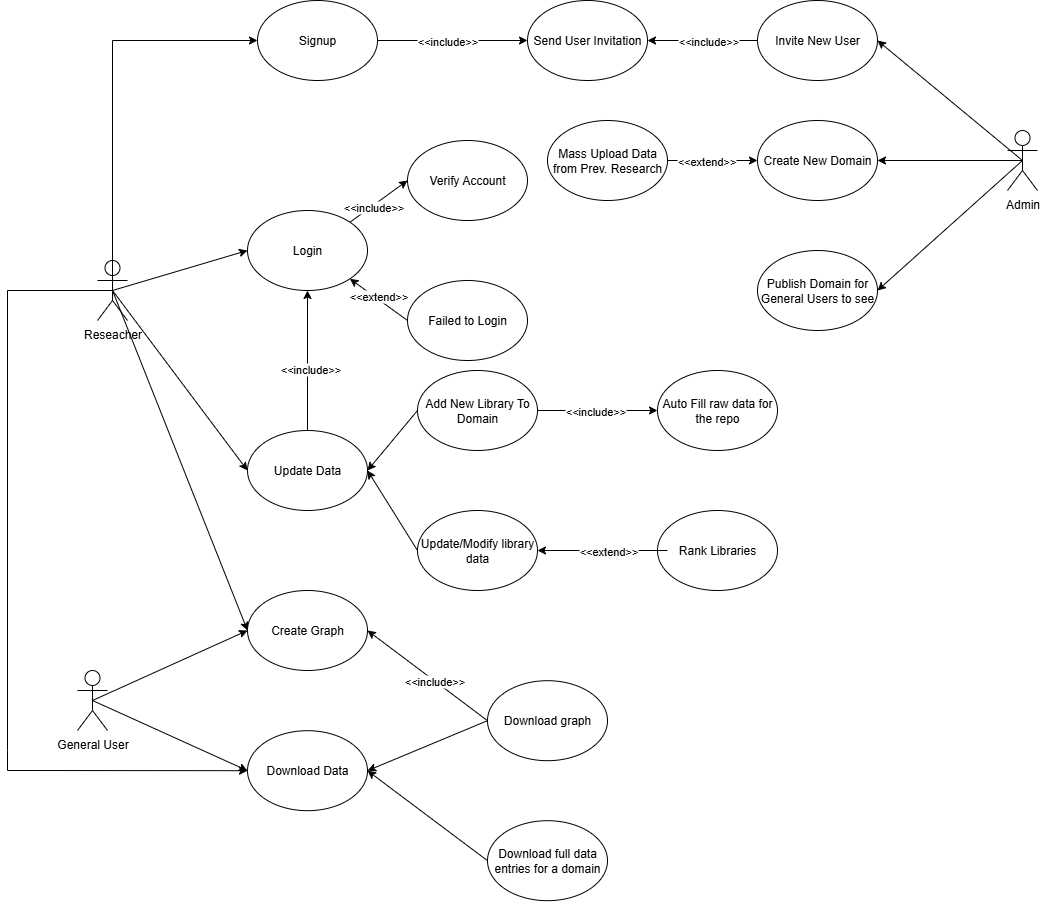
\includegraphics{usecase.png}\begin{figure}[H]
    \centering
    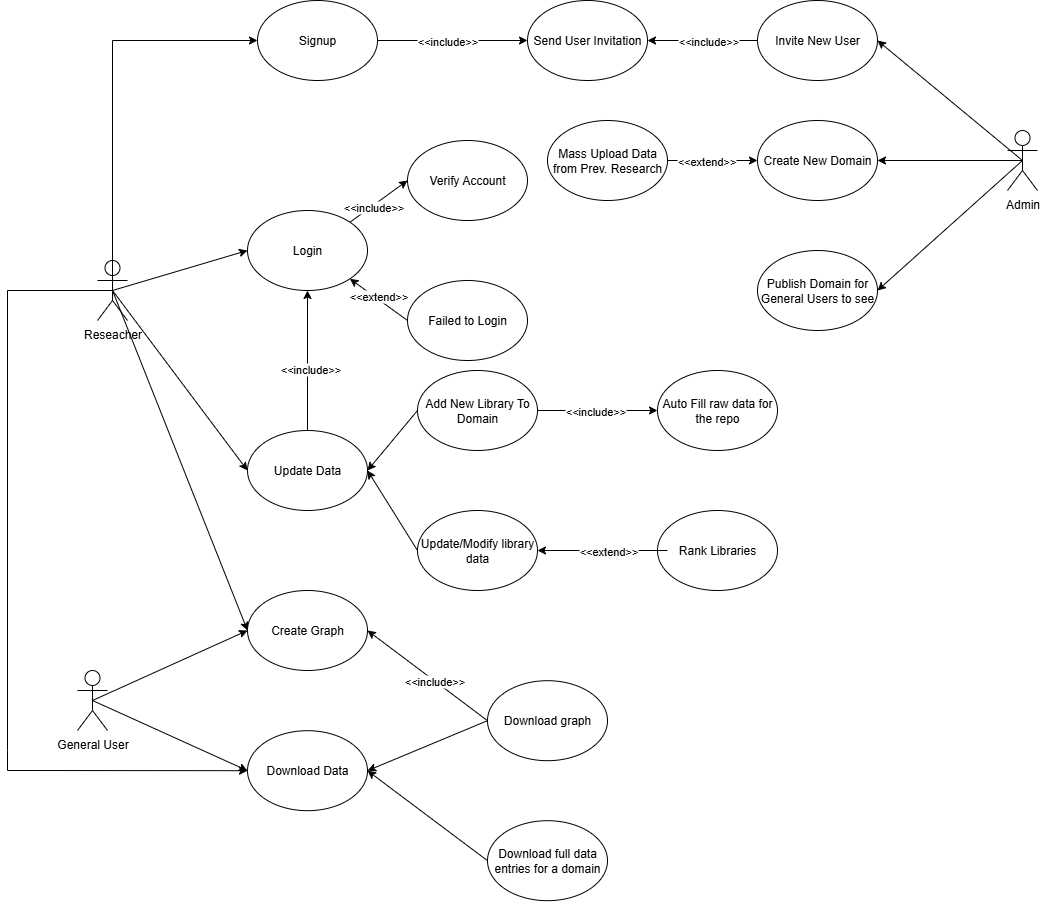
\includegraphics[scale=0.45] {usecase.png}
\end{figure}


\section{Functional Requirements}
\subsection{Functional Requirements}
\begin{enumerate}[label=\thesubsection-\arabic*]
  \item The Admin will be able to extend an invitation to new researchers via the website, using the researcher's email address.
  \item Researchers will be able to sign up using their invited email. The process requires email validation and the creation of a unique username and password.
  \item The system will allow Admin and Researchers to securely log in using their email and password.
  \item Users will be able to reset their password after validating their email address.
  \item Admin can create domains, using a unique domain name and optionally a short description.
  \item Admin can publish a domain, once research is completed, for anyone to see and download data collected.
  \item Researchers can add/modify data/libraries of existing domains, and download data/graphs regardless of completion status.
  \item The system must validate all user input upon addition or update (e.g., ensuring numeric fields are numbers, dates are valid, and text limits are met).	
  \item The system must allow a Admin to bulk upload library and metric data using a predefined Excel template. The system must report detailed errors for any records that fail validation, such as feature names not being in the scope or wrong data type for a column.
  \item When a Researcher enters a public GitHub URL for a library, the system must call the GitHub API to automatically retrieve and populate specific data points, such as the Repository Creation Date and the Last Commit Date.
  \item The system must display a complete list of all metrics and their definitions for a selected domain.
  \item The system will rank the libraries within a domain using the Analytical Hierarchy Process (AHP) and display the calculated results.
  \item Users must be able to select a domain → libraries → metrics → graph type to visualize differences in libraries using comparative graphs.
  \item All users will be able to download the collected data for a specific scope in JSON, Excel, or LaTeX code formats to their device.
  \item Users must be able to download any generated graph, with the option to save it as a PNG file.
\end{enumerate}

\section{Look and Feel Requirements}
\subsection{Appearance Requirements}
\begin{enumerate}[label=\thesubsection-\arabic*]
  \item The application will maintain a consistent visual hierarchy where primary action buttons (e.g., "Save," "Create New Domain") are visually distinct.
  \item The system must be fully responsive and function correctly on standard desktop monitors and laptops.
  \item Data visualization and editing displays must prioritize information density while remaining readable. Tables should have alternating row colors (zebra striping) to help tracking.
  \item The main user dashboard should provide a clear, high-level overview of active domains and tasks, with minimal visual clutter.
  \item Ensure all required input fields are clearly identified (e.g., with an asterisk). Input forms must give real-time feedback, such as a green checkmark for acceptable input and a red boundary for errors.
  \item All error messages (system errors, validation problems) must be clear, short, and contain practical guidance for resolving the problem.
\end{enumerate}
\subsection{Style Requirements}
\begin{enumerate}[label=\thesubsection-\arabic*]
  \item The system must use a single, consistent style of icons (e.g., solid, outline, or filled) for all navigational elements, actions, and status indicators.
  \item Graphs must use minimalist design to prioritize data readability. Axes and labels must be clear and legible.
  \item Font sizing must follow a defined scale (e.g., large for titles, medium for body text, small for captions) and remain consistent on all screens.
\end{enumerate}

\section{Usability and Humanity Requirements}
\subsection{Ease of Use Requirements}
\begin{enumerate}[label=\thesubsection-\arabic*]
  \item The primary navigational structure should be clearly defined and constantly available, with no prior training required for basic data viewing and download.
  \item Each library metric must have help icon that would tell the user what data type would be accepted.
  \item All errors will give clear and concise explanation.
\end{enumerate}
\subsection{Personalization and Internationalization Requirements}
N/A
\subsection{Learning Requirements}
\begin{enumerate}[label=\thesubsection-\arabic*]
  \item The system must contain a brief lesson or guide that explains the precise steps for Bulk Data Upload and the AHP Ranking process and is available from the appropriate screens.
  \item All words referring to research entities (Domain, Library, Metric) must be used consistently across the interface and documentation.
\end{enumerate}
\subsection{Understandability and Politeness Requirements}
\begin{enumerate}[label=\thesubsection-\arabic*]
  \item The system must contain a brief lesson or guide that explains the precise steps for Bulk Data Upload and the AHP Ranking process and is available from the appropriate screens.
  \item All words referring to research entities (Domain, Library, Metric) must be used consistently across the interface and documentation.
  \item All system-generated error messages will be clear, use non-technical language, and suggest a simple course of corrective action
\end{enumerate}
\subsection{Accessibility Requirements}
\begin{enumerate}[label=\thesubsection-\arabic*]
  \item Critical status indicators and data visualizations must convey meaning through patterns or text labels in addition to color.
  \item Users must be able to change font size using regular browser options (up to 200\%) without losing information or functionality.
\end{enumerate}

\section{Performance Requirements}
\subsection{Speed and Latency Requirements}
\begin{enumerate}[label=\thesubsection-\arabic*]
  \item All key data viewing and dashboard pages must load completely and become interactive within 3 seconds.
  \item The system must finish the AHP ranking calculation for a standard domain in less than ten seconds.
\end{enumerate}
\subsection{Safety-Critical Requirements}
\begin{enumerate}[label=\thesubsection-\arabic*]
  \item The system will encrypt all user passwords.
  \item If there have been multiple failed attempts to login to an existing account the user must be notified and lock account.
  \item The system will ensure that only researchers modify data.
\end{enumerate}\subsection{Precision or Accuracy Requirements}
\begin{enumerate}[label=\thesubsection-\arabic*]
  \item All data  that the system automatically filled out, must be 100\% accurate.
\end{enumerate}
\subsection{Robustness or Fault-Tolerance Requirements}
\begin{enumerate}[label=\thesubsection-\arabic*]
  \item The system must implement graceful error handling, ensuring that a failure in one function (e.g., a failed GitHub API call) does not crash the entire application or disrupt other users.
  \item The system must use database transactions to ensure that data modifications are atomic, if an update operation fails in the middle, the data must be returned to its last validated state.
\end{enumerate}
\subsection{Capacity Requirements}
\begin{enumerate}[label=\thesubsection-\arabic*]
  \item The system must be able to accommodate up to 20 concurrent active users (logged in and doing operations) with no visible performance decrease.
  \item The database must be constructed to accommodate at least 10 different study domains.
\end{enumerate}
\subsection{Scalability or Extensibility Requirements}
\begin{enumerate}[label=\thesubsection-\arabic*]
  \item The system architecture must clearly divide the Data Management/Storage layer from the Analysis/Visualization layer so that either component may be improved or replaced independently.
  \item The authentication and authorization system must be adaptable enough to accommodate additional user roles (e.g., "Guest Analyst") and specialized rights without requiring code changes to core operations.
\end{enumerate}
\subsection{Longevity Requirements}
\begin{enumerate}[label=\thesubsection-\arabic*]
  \item The system must be capable of running without the requirement for maintenance for two years. 
\end{enumerate}

\section{Operational and Environmental Requirements}
\subsection{Expected Physical Environment}
\lips
\subsection{Wider Environment Requirements}
\lips
\subsection{Requirements for Interfacing with Adjacent Systems}
\lips
\subsection{Productization Requirements}
\lips
\subsection{Release Requirements}
\lips

\section{Maintainability and Support Requirements}
\subsection{Maintenance Requirements}
\lips
\subsection{Supportability Requirements}
\lips
\subsection{Adaptability Requirements}
\lips

\section{Security Requirements}
\subsection{Access Requirements}
\lips
\subsection{Integrity Requirements}
\lips
\subsection{Privacy Requirements}
\lips
\subsection{Audit Requirements}
\lips
\subsection{Immunity Requirements}
\lips

\section{Cultural Requirements}
\subsection{Cultural Requirements}
\lips

\section{Compliance Requirements}
\subsection{Legal Requirements}
\lips
\subsection{Standards Compliance Requirements}
\lips

\section{Open Issues}
\lips

\section{Off-the-Shelf Solutions}
\subsection{Ready-Made Products}
\lips
\subsection{Reusable Components}
\lips
\subsection{Products That Can Be Copied}
\lips

\section{New Problems}
\subsection{Effects on the Current Environment}
\lips
\subsection{Effects on the Installed Systems}
\lips
\subsection{Potential User Problems}
\lips
\subsection{Limitations in the Anticipated Implementation Environment That May
Inhibit the New Product}
\lips
\subsection{Follow-Up Problems}
\lips

\section{Tasks}
\subsection{Project Planning}
\lips
\subsection{Planning of the Development Phases}
\lips

\section{Migration to the New Product}
\subsection{Requirements for Migration to the New Product}
\lips
\subsection{Data That Has to be Modified or Translated for the New System}
\lips

\section{Costs}
\lips
\section{User Documentation and Training}
\subsection{User Documentation Requirements}
\lips
\subsection{Training Requirements}
\lips

\section{Waiting Room}
\lips

\section{Ideas for Solution}
\lips

\newpage{}
\section*{Appendix --- Reflection}

The purpose of reflection questions is to give you a chance to assess your own
learning and that of your group as a whole, and to find ways to improve in the
future. Reflection is an important part of the learning process.  Reflection is
also an essential component of a successful software development process.  

Reflections are most interesting and useful when they're honest, even if the
stories they tell are imperfect. You will be marked based on your depth of
thought and analysis, and not based on the content of the reflections
themselves. Thus, for full marks we encourage you to answer openly and honestly
and to avoid simply writing ``what you think the evaluator wants to hear.''

Please answer the following questions.  Some questions can be answered on the
team level, but where appropriate, each team member should write their own
response:


\begin{enumerate}
  \item What went well while writing this deliverable? 
  \item What pain points did you experience during this deliverable, and how did
  you resolve them?
  \item How many of your requirements were inspired by speaking to your
  client(s) or their proxies (e.g. your peers, stakeholders, potential users)?
  \item Which of the courses you have taken, or are currently taking, will help
  your team to be successful with your capstone project.
  \item What knowledge and skills will the team collectively need to acquire to
  successfully complete this capstone project?  Examples of possible knowledge
  to acquire include domain specific knowledge from the domain of your
  application, or software engineering knowledge, mechatronics knowledge or
  computer science knowledge.  Skills may be related to technology, or writing,
  or presentation, or team management, etc.  You should look to identify at
  least one item for each team member.
  \item For each of the knowledge areas and skills identified in the previous
  question, what are at least two approaches to acquiring the knowledge or
  mastering the skill?  Of the identified approaches, which will each team
  member pursue, and why did they make this choice?
\end{enumerate}


\end{document}